\documentclass[
    fontsize=12pt,
    parskip=half
]{scrartcl}

\usepackage[utf8]{inputenc}
\usepackage[T1]{fontenc}
\usepackage{microtype}
\usepackage{graphicx}
\usepackage[ngerman]{babel}

% Schriftart FiraSans https://tug.org/FontCatalogue/firasanslight/
\usepackage[sfdefault,light]{FiraSans}
\usepackage[T1]{fontenc}
\renewcommand*\oldstylenums[1]{{\firaoldstyle #1}}

\usepackage{tikz}
\usetikzlibrary{positioning,arrows,calc,matrix}
\usepackage{tabularx}
\newcolumntype{R}{>{\raggedright\arraybackslash}X}

% Funktionale Anforderung
\newcommand\fa{}

\title{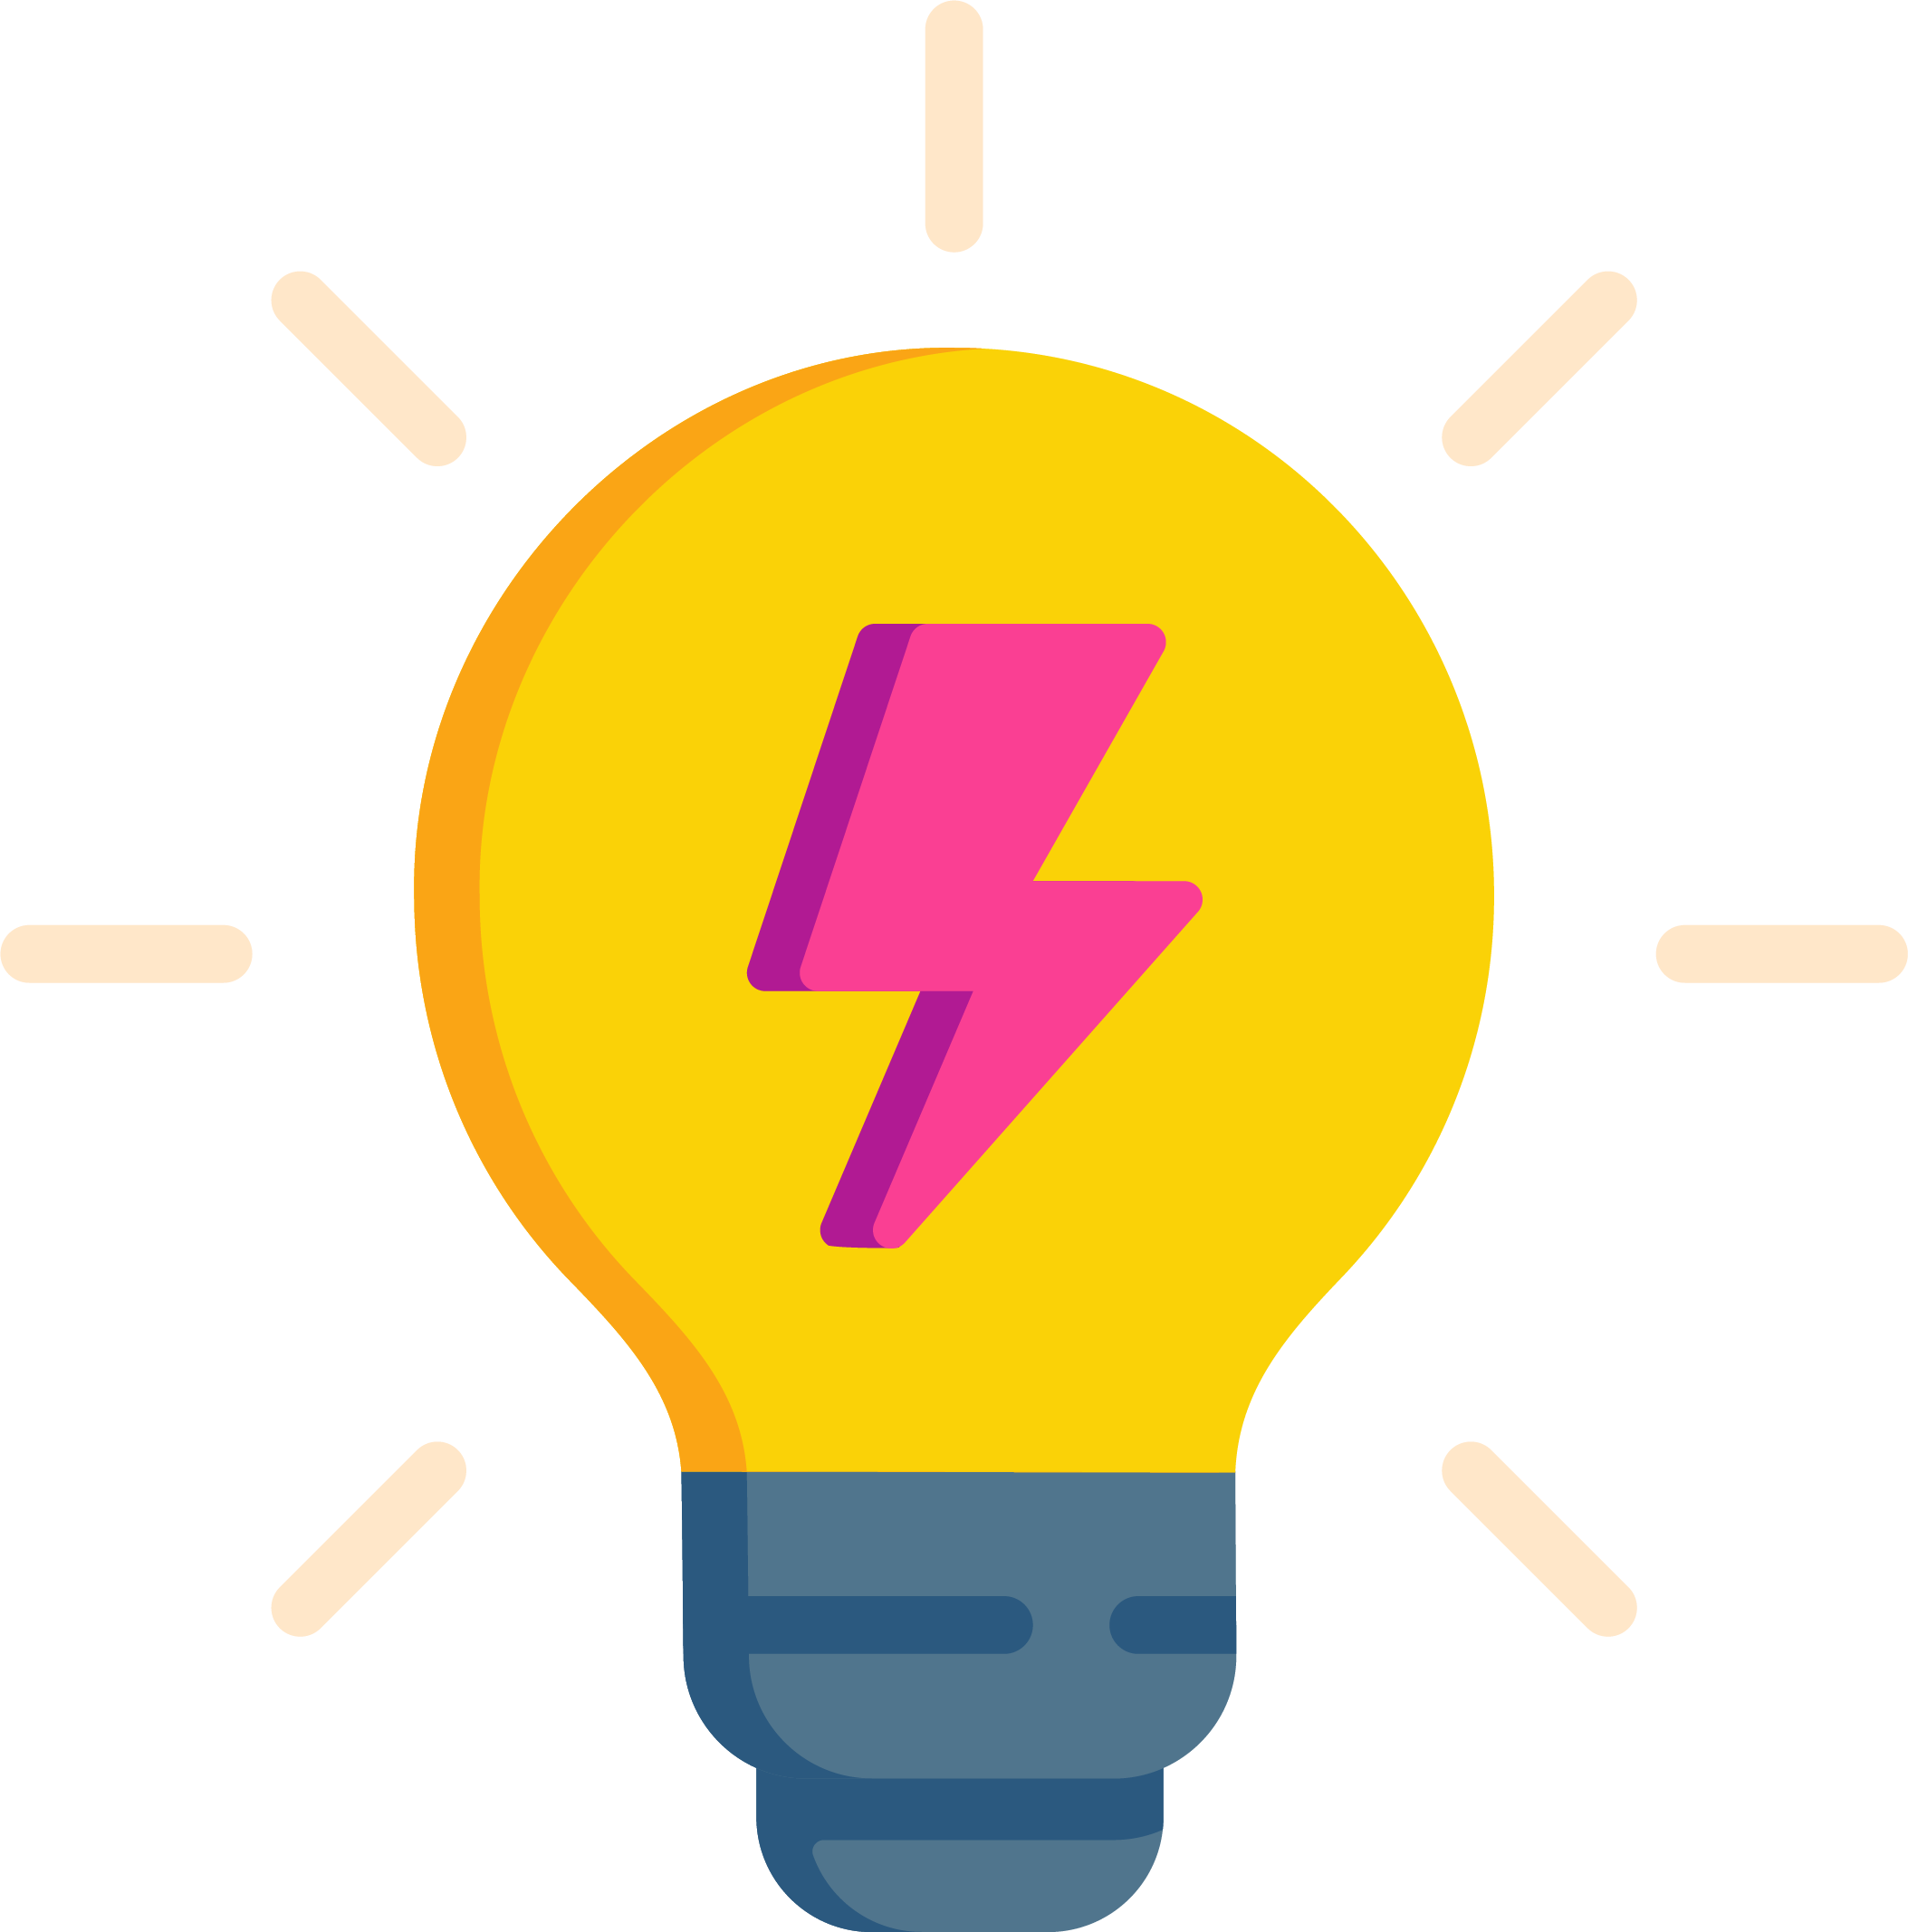
\includegraphics[height=25mm]{icon.png}\\Projekt \emph{Smart Energy}}
\author{HB Solutions GbR}

\begin{document}
\maketitle

\section{Einführung}
In diesem Dokument werden die Anforderungen für das Projekt \emph{Smart Energy}, in Auftrag gegeben durch die Rüdensche Windenergie AG (RWE) und durchgeführt von der HB Solutions GbR, aufgestellt.
\emph{Smart Energy} sieht vor, eine zentrale Kraftwerkssteuerung für Versorger und Verbraucher in einem Stromnetz zu erstellen.
Die Versorger reichen von einer Vielzahl an unterschiedlichen Kraftwerken wie etwa für Solar-, Wind- und Biomasseenergie.
Der Kunde RWE bedient sowohl Haushalte als auch Unternehmen als Verbraucher.
Stromspeicher sieht der Kunde nicht in der Kraftwerkssteuerung vor.
Die Kraftwerke werden zunächst simuliert, damit die Software zunächst vollständig fertiggestellt und getestet werden kann, bevor sie in einer Realumgebung eingesetzt wird.

\section{Anforderungsanalyse}
Das Projekt setzt sich aus mehreren Komponenten zusammen.
Dabei steht im Zentrum die Kraftwerkssteuerung.
Weitere Komponenten sind Erzeuger und Verbraucher.
Ferner können weitere Komponenten wie Browser oder Energieversorger über definierte Schnittstellen mit dem System interagieren (z.B. historische Daten abfragen).

\subsection{Kraftwerkssteuerung}
Die zentrale Kraftwerkssteuerung koordiniert Erzeuger und Verbraucher.
Zusätzlich soll die zentrale Kraftwerkssteuerung in der Lage sein, per TCP/HTTP mit jedem beliebigen Webbrowser zu kommunizieren.
Dafür stellt die Kraftwerkssteuerung einen HTTP-Server mit einer REST-API zur Verfügung, die mindestens \texttt{GET}-Anfragen unterstützt.
Über diese REST-API können dann externe Komponenten wie ein Webbrowser auf die Steuerung zugreifen.
Alternativ dazu, soll die Kraftwerkssteuerung selbst auch per RPC-Schnittstelle konfigurierbar sein, die externe Clients wie Energieversorger nutzen können.
Informationen der Erzeuger und Verbraucher werden sowohl vorerst per UDP, als auch später per MQTT empfangen. 

\subsection{Erzeuger / Verbraucher}
Die Erzeuger und Verbraucher teilen ihre Informationen mit der Kraftwerkssteuerung vorerst per UDP, im späteren Verlauf des Projekts aber auch via MQTT.
Die Konfiguration der Komponenten durch die Kraftwerkssteuerung soll jedoch per RPC geschehen.
Dabei ist darauf zu achten, dass Versorger und Verbraucher klar identifizierbar sind, die Art des Teilnehmers bekannt ist, der Stromverbrauch/-erzeugung in kW angegeben ist und er per UDP mit der Zentralen Kraftwerkssteuerung kommuniziert. 
Der Kunde sieht für die Simulation mindestens vier Verbraucher/Erzeuger vor, darunter mindestens ein Verbraucher. 
Zum verbesserten Testen soll der Verbrauch bzw. die erzeugte Menge  künstlich variieren können.


% \subsection{Nicht-funktionale Anforderungen}
% Das Projekt wird in C++ programmiert. Da die Vorgabe des Kunden ist, in C++ oder in Java zu programmieren.  

\subsection{Funktionale Anforderungen}

\begin{enumerate}
    \item Software für Energieversorger sowie -verbraucher erstellen, die folgende Informationen übermitteln:
    \begin{enumerate}
        \item Art des Teilnehmers
        \item Eindeutige ID oder Name zur klaren Identifikation
        \item Aktuelle Strommenge in kW (variiert je nach Versorger und Verbraucher)
        \item Kommunikation über UDP und später MQTT
        \item Steuerung über RPC
    \end{enumerate}
    \item Es werden mind 4. unabhängige Erzeuger/Verbraucher erstellt (davon mind. 1 Verbraucher)
    \item Software für Zentrale Kraftwerkssteuerung (ZK) erstellen mit folgenden Anforderungen:
    \begin{enumerate}
        \item Horizontal skalierbar
        \item UPD Schnittstelle (später MQTT) für Verbraucher/Erzeuger
        \item REST-Schnittstelle, die mindestens \texttt{GET}-Anfragen verarbeiten kann
        \item Eigene HTTP-Server-Implementierung
        \item RPC-Schnittstelle für externen Client implementieren
    \end{enumerate}
    \item Software für externen Client erstellen
    \begin{enumerate}
        \item Kann RPC-Schnittstelle von ZK nutzen
    \end{enumerate}
\end{enumerate}

\subsection{Nicht-funktionale Anforderungen}
\begin{enumerate}
    \item Programmiersprache ist C++
    \item Gitlab CI (Docker und Docker-compose)
    \item Clean Code
    \item Hygiene des Git-Repositories
    \item Dokumentation
    \item Lizenzen
    \item \texttt{Dockerfile} und \texttt{docker-compose.yml} Beispiele
    \item HTTP selbst implementiert
\end{enumerate}

\section{Systemdesign}
\begin{center}
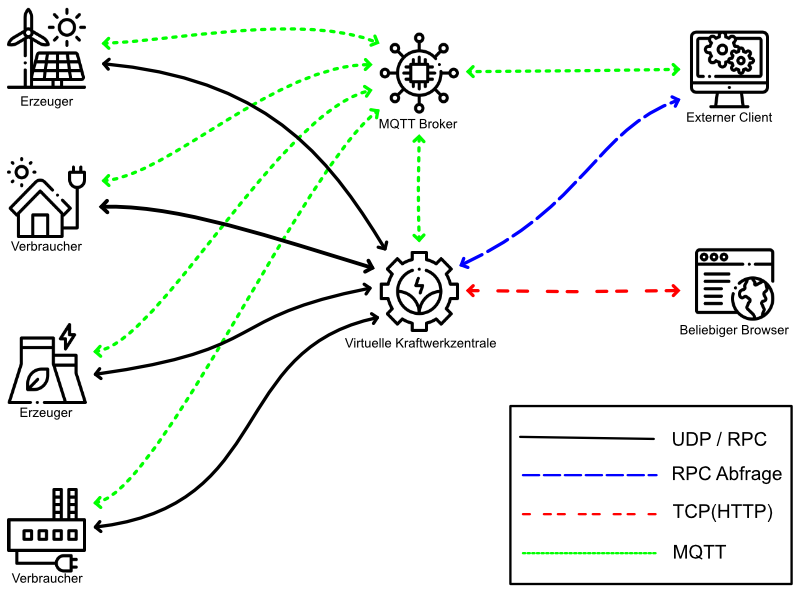
\includegraphics[width=\textwidth]{Systemdesign.png}
\end{center}

\section{Testing}

\subsection{Funktionale Tests}
    \begin{itemize}
        \item Können UDP Packete von jedem Erzeuger zur zentralen Kraftwerkssteuerung gesendet werden?
        \item Funktioniert die RPC Verbindung zwischen Verbraucher/Erzeuger und Kraftwerkssteuerung?
        \item Kann die Kraftwerkssteuerung von Chromium und Firefox erreicht werden?
        \item Können Erzeuger/Verbraucher eindeutig erkannt werden?
        \item Ist der aktuelle Stromverbrauch/-erzeugung variierbar?
        \item Kann der Client per RPC die Kraftwerkssteuerung konfigurieren?
    \end{itemize}
\subsection{Nicht-Funktionale Tests}
    \begin{itemize}
        \item Ist das Prgramm in C++ geschrieben
        \item Ist eine aktuelle Version des Projekts bei Abschluss auf dem Masterbranch?
        \item Lässt sich das Projekt mit einem Befehl deployen?
        \item Wird das Projekt über eine Pipeline gebaut?
        \item Ist das Projekt dokumentiert?
        \item Ist HTTP selbst implementiert?
        \item Liegt ein \texttt{Dockerfile} vor?
        \item Liegt dem Projekt eine Lizenz bei?
        \item Wurden Coding Best-Practices eingehalten?
    \end{itemize}

\subsection{Performance-Tests}
\begin{itemize}
    \item Verarbeitungsdauer von eintreffenden UDP-Paketen
    \item Belastungsgrenze UDP-Pakete pro Sekunde
    \item Belastungsgrenze MQTT-Nachrichten pro Sekunde
    \item Maximale Anzahl an verbundenen Verbraucher und Erzeugern über RPC
\end{itemize}

\section{Projektplan}
\begin{tabularx}{\textwidth}{|l|R|}
\hline
\textbf{Datum} & \textbf{Meilenstein} \\
\hline
Praktikum 1 & Planung des Projekts \\
\hline
Praktikum 2 & Kraftwerkssteuerung + Webserver\linebreak
    Verbraucher/Erzeuger und\linebreak
    funktionierende Kommunikation zwischen Komponenten \\
\hline
Praktikum 3 & 
    Einfügen von RPC Schnittstellen\linebreak
    Testen der RPC Schnittstellen von Seiten Client und Kraftwerkssteuerung \\
\hline
Praktikum 4 & 
    Einführen eines MQTT-Broker\linebreak
    Performancetest und Vergleich MQTT zu UDP \\
\hline
Praktikum 5 & 
    Kraftwerkssteuerung horizontal erweitern \\
\hline
Praktikum 6 &
    ggf. Abschlussprotokoll \\
\hline
\end{tabularx}

\section{Deployment}
Um das Projekt auszurollen, wird die HB Solutions GbR CI in Gitlab nutzen. 
In dieser werden Tests automatisch ausgeführt und die Entwickler stellen sicher, dass zu jedem Zeitpunkt ein lauffähiges System existiert.

Lokal, der Simulation dienend, stellt das Projekt eine \texttt{docker-compose.yml}-Datei zur Verfügung, um eine Testumgebung aufzusetzen.
Für das spätere Deployment in der tatsächlichen Umgebung ist eine Ansible-Role angedacht.

\end{document}

\section{Änderungsprotokoll}
-
